\documentclass[12pt,a4paper,]{adreport}
\usepackage[T1]{fontenc}
\usepackage{lmodern}
\usepackage{amssymb,amsmath}
\usepackage{ifxetex,ifluatex}
\usepackage{lscape}
\usepackage{fixltx2e} % provides \textsubscript
% use upquote if available, for straight quotes in verbatim environments
\IfFileExists{upquote.sty}{\usepackage{upquote}}{}
\ifnum 0\ifxetex 1\fi\ifluatex 1\fi=0 % if pdftex
  \usepackage[utf8]{inputenc}
\else % if luatex or xelatex
  \ifxetex
    \usepackage{mathspec}
    \usepackage{xltxtra,xunicode}
  \else
    \usepackage{fontspec}
  \fi
  \defaultfontfeatures{Mapping=tex-text,Scale=MatchLowercase}
  \newcommand{\euro}{€}
\fi
% use microtype if available
\IfFileExists{microtype.sty}{\usepackage{microtype}}{}
\usepackage{longtable,booktabs}
\usepackage{graphicx}
% Redefine \includegraphics so that, unless explicit options are
% given, the image width will not exceed the width of the page.
% Images get their normal width if they fit onto the page, but
% are scaled down if they would overflow the margins.
\makeatletter
\def\ScaleIfNeeded{%
  \ifdim\Gin@nat@width>\linewidth
    \linewidth
  \else
    \Gin@nat@width
  \fi
}
\makeatother
\let\Oldincludegraphics\includegraphics
{%
 \catcode`\@=11\relax%
 \gdef\includegraphics{\@ifnextchar[{\Oldincludegraphics}{\Oldincludegraphics[width=\ScaleIfNeeded]}}%
}%
\ifxetex
  \usepackage[setpagesize=false, % page size defined by xetex
              unicode=false, % unicode breaks when used with xetex
              xetex]{hyperref}
\else
  \usepackage[unicode=true]{hyperref}
\fi
\hypersetup{breaklinks=true,
            bookmarks=true,
            pdfauthor={},
            pdftitle={},
            colorlinks=true,
            citecolor=blue,
            urlcolor=blue,
            linkcolor=magenta,
            pdfborder={0 0 0}}
\urlstyle{same}  % don't use monospace font for urls
\usepackage[normalem]{ulem}
% avoid problems with \sout in headers with hyperref:
\pdfstringdefDisableCommands{\renewcommand{\sout}{}}
\setlength{\parindent}{0pt}
\setlength{\parskip}{6pt plus 2pt minus 1pt}
\setlength{\emergencystretch}{3em}  % prevent overfull lines
\setcounter{secnumdepth}{5}

\author{}
\date{}

\begin{document}

{
\hypersetup{linkcolor=black}
\setcounter{tocdepth}{2}
\tableofcontents
}
\chapter{Introduction}\label{introduction}

Note: In this draft version, crossed-out text represent notes and
guidance from the intranet site which have not yet been removed.

\section{Overall Aim of the Project}\label{overall-aim-of-the-project}

\section{Problem Description}\label{problem-description}

Data storage has increasingly become the responsibility of
special-interest corporations, who leverage their existing massive
server infrastructure (or server infrastructure subcontractors) to
reduce the legwork for ordinary consumers wishing to back up their data.
The concept of the `cloud' was invented to further psychologically
bolster these datacentres; a fluffy, harmless-sounding term referring to
some ethereal space where all your data safely resides.

The reality, as ever, is much less reassuring. Corporations want your
data data because, as the old saying goes, information is power. The
purpose of this `cloud' is not to secure average users' data but to
generate Big Data (another modern term which refers to a different
aspect of the same thing, this one coined by and for cardboard-cutout
nonpeople, greed in suits and economists with dollar signs for eyes),
which can be analysed statistically at massive scale, in order to better
improve the company's profit techniques. Information of this type is
available at such scale that new psychological techniques can be devised
to coerce users, such as gamification. More personal messages can be
created, using well-educated guesses about the interests and
demographics of a portion of the company's audience.

It can be almost impossible to put the cat back into the bag once
corporation(s) have dug their heels into an area of human interest --
barring massive governmental intervention, such as
internationally-backed legislation. However some things have been shown
to be easier to fix than others. The Open Source movement has shown that
by initially appealing to users' greed by offering something for which
they would otherwise have to pay money for free, it is possible to draw
non-technical users away from for-profit services. The effectiveness of
doing this is also strongly influenced by the presentation and appeal of
the software, which modern businesses have evolved to take very
seriously, creating an entire field called `brand management'.

Computers have made it convenient to store all our important family data
digitally. Family photos, videos, genealogy records, old family recipes;
they all take less physical space on a disk, and can be copied easily
for anyone interested. However, digital data is at risk of loss
(flooding, fire and theft being the most often mentioned), and most
homes don't have the infrastructure in place to preserve their family's
unique data long-term. Lay users often have little or no idea about
where or how their data is stored (on their computer or on the
Internet), whether it is safe and whether their rights to it have been
compromised by a Terms Of Service agreement (TOS).

\section{Aspects of the Background}\label{aspects-of-the-background}

\begin{itemize}
\itemsep1pt\parskip0pt\parsep0pt
\item
  why the project is worth doing
\item
  how the project may be useful or helpful for others
\end{itemize}

\section{Project Goals}\label{project-goals}

\begin{itemize}
\itemsep1pt\parskip0pt\parsep0pt
\item
  Develop a distrbuted backup syncing program, autonomous enough for
  non-technical users to be able to use
\item
  Design and implement an efficient file synchronisation protocol to
  support this
\item
  Design and implement a new serialisation suite which is both efficient
  and succinct for our purposes

  \begin{itemize}
  \itemsep1pt\parskip0pt\parsep0pt
  \item
    Write a language-agnostic specification
  \item
    Implement the specification in Java
  \end{itemize}
\end{itemize}

brief chapter-by-chapter overview of the rest of the report

Unique data collections such as photos are often stored on a physical
medium which is vulnerable to damage or corruption. CDs are damaged by
heat, light and wear and tear. When this storage fails (mobile phones
are lost, old PCs break down or are replaced due to age, without
sufficiently diligent data transferral), often the user unwittingly
throws away or loses many years of irreplaceable data.

Lost laptops and pen drives cause frequent loss of important data. Old
PCs being replaced cause families to throw away accumulated personal
data, without realising what is stored locally rather than on the
Internet -- lack of understanding causes further personal data loss upon
hardware failure.

The backup strategy often lauded as the most prudent follows the 3-2-1
strategy: 3 copies, on 2 different storage media, 1 offsite
backup.\footnote{``Backups with the 3-2-1 rule''
  (http://blog.wisefaq.com/2010/01/05/backups-with-the-3-2-1-rule/)
  (accessed 25/06/2014)} This is an ideal, but is extremely difficult
for a home user to set up and maintain, without corporate resrouces at
their disposal. For instance:

\begin{itemize}
\itemsep1pt\parskip0pt\parsep0pt
\item
  How does one set up backups in different locations?
\item
  How does one sync updates to each offsite copy?
\end{itemize}

This project aims to answer these questions with a software solution,
reducing the risk of data loss for families (and other groups with an
interest in long-term data preservation) due to lack of sufficient
knowledge and/or funds for more thorough backup solutions, without
relying on a third party service that has ulterior motives.

\section{Main Project Features}\label{main-project-features}

Distribackup will watch the contents of a directory, and keep its
contents synced with identical directories on other computers. Because
there is no authoritative server broadcasting updates to parties,
syncing will use a distributed model to propagate changes. In order to
expedite large file transfers (which are likely in the primary use
case), a differencing algorithm will be used to only send pieces of
files that have changed with an update.

This report will describe why this software is needed, comparing it to
related work, and showing how this project can build on this work. It
will then describe the proposed programme of work to be undertaken in
order to complete the bare-bones implementation offered here; continuing
by laying out the sub-components of the software, their purposes, and
how they fit together to complete the end goal. The methodology will
then be explained, describing what software development techniques will
be used during the project. This will lead into the proposed evaluation
methodology, and how research will be carried out.

The expected timeline for this work will then be described in detail,
accompanied by a Gantt chart showing this visually. The report will then
finish by listing the resources required in order for it to be
completed, and a list of references used.

\chapter{Background}\label{background}

\subsection{Any improvements that your system
offers}\label{any-improvements-that-your-system-offers}

\subsection{shortcomings that your work addresses, and so
on}\label{shortcomings-that-your-work-addresses-and-so-on}

\section{Justify your choice of platform, software, solution
etc}\label{justify-your-choice-of-platform-software-solution-etc}

\section{Summary of technical problems and
approaches}\label{summary-of-technical-problems-and-approaches}

More than ever before there is a need for long-term backup software
which is accessible for everyone. There are now years' worth of data
stored digitally which record milestones in peoples' lives, all stored
on machines they don't fully understand. This lack of understanding will
eventually lead to data loss, but not everyone should be a computer
scientist, or even technically capable. But everyone should be able to
preserve their family's history.

\section{Relevant work and/or existing related
systems}\label{relevant-work-andor-existing-related-systems}

\subsection{implications for this
project}\label{implications-for-this-project}

This is by no means an exhaustive list, but discusses the most relevant
existing solutions (at time of writing), and describes how Distribackup
differs or extends from them.

\subsection{Bit-Torrent}\label{bit-torrent}

\begin{itemize}
\itemsep1pt\parskip0pt\parsep0pt
\item
  Collection contents cannot be changed after torrent creation
\item
  Unsecure by design (IP addresses and ISP hostnames are broadcast and
  used as identities)
\item
  Nowadays highly stigmatised; associated with illegal activity
  (copyright theft) in public consciousness
\end{itemize}

\subsection{Bit-Torrent Sync}\label{bit-torrent-sync}

\begin{itemize}
\itemsep1pt\parskip0pt\parsep0pt
\item
  Not open source, despite the company's most famous software's
  background
\item
  Not originally designed for optimal data transfer

  \begin{itemize}
  \itemsep1pt\parskip0pt\parsep0pt
  \item
    Differential techniques not used
  \end{itemize}
\item
  Without file differencing, their protocol is inefficient for updates
  to large files
\item
  Use cases could be very similar to Distribackup's
\end{itemize}

\subsection{Syncthing}\label{syncthing}

http://syncthing.net/

\begin{itemize}
\itemsep1pt\parskip0pt\parsep0pt
\item
  No longer part of ind.ie
\end{itemize}

\subsection{Git}\label{git}

Git was designed from the ground-up by Linus Torvalds as a decentralised
version control system, competing with Subversion, CVS and Mercurial.

Most developer's contact with Git is through a centralised,
authoritative repository, usually hosted by a company such as GitHub or
Bit Bucket. However, Git is able to function equally well as a
standalone repository or for managing difference relationships between
disparate but equally authoritative collections of copies.

Central, authoritative copies of files can be useful when attempting to
establish precedence, or evolve a single product towards completion,
allowing users to exchange changes with each other through a single
point of contact: the Master. This is much easier to conceptualise for
users than communicating changes between slightly different
repositories, and easier for maintaining a distributable copy for new
entrants.

\begin{itemize}
\item
  Updates require user intervention git updates need to be synced by
  user, using command line or separate GUI
\item
  Not automatic
\item
  Very hands-on; cannot fire-and-forget
\item
  Large vocabulary of commands to learn
\item
  Assumption of user = programmer

  \begin{itemize}
  \itemsep1pt\parskip0pt\parsep0pt
  \item
    unexplained technical concepts
  \end{itemize}
\item
  Git is not visible to end-users: its intended audience is developers,
  and its steep learning curve (tens of commands to learn each with its
  own set of single-character optional parameters; a new mental model
  for manipulating `staged' files which are `indexed') would prevent its
  adoption by non-programmer power users
\item
  Existing GUIs for git are unfinished, non-free, buggy or as confusing
  as the command line interface, with none of the portability.
\item
  Git is much more complex than is necessary for our task
\end{itemize}

\subsection{Git-Annex}\label{git-annex}

Git-Annex, and its GUI front-end Git-Annex Assistant allow the user to
manage collections of large files using git, without checking the file
contents into git.\footnote{Joey Hess, ``Git Annex''
  (http://git-annex.branchable.com/) (Accessed 25/06/2014)}

Git-annex is aimed towards a more technically literate user. Also, as
with Sparkleshare, a central server is needed to manage and distribute
changes between different storage nodes.

\subsection{Ceph}\label{ceph}

Ceph is a distributed file system. Ceph is aimed more at technically
proficient users and industry professionals.

\subsection{Tahoe-LAFS}\label{tahoe-lafs}

Tahoes-LAFS (Least Authority File system) is an open source distributed
file system, focused on providing self-hosted cloud storage that is
resistant to attack.\footnote{``Tahoe one-page summary''
  (https://tahoe-lafs.org/trac/tahoe-lafs/browser/trunk/docs/about.rst)
  (accessed 24/06/2014)} This, again, is aimed much more at system
administrators and other professionals with an understanding of the
area.

\subsection{Sparkleshare}\label{sparkleshare}

Sparkleshare{[}sparkleshare{]} is also an open-source cloud syncing
solution with the intention of providing an alternative to DropBox.

Sparkleshare is backed by Git and SSH, and is well suited to managing a
collection of many regularly-changing small (mostly text) files which
are edited by a group, such as in a software development team.\footnote{http://sparkleshare.org/\#good
  (accessed 25/06/2014)} However, by its own admission Sparkleshare is
not well-suited to full-computer backups, or for storing large archives
of binary data such as photos and videos.\footnote{http://sparkleshare.org/\#bad
  (accessed 25/06/2014)} Sparkleshare also relies on a centralised
server to manage backups, which introduces an infrastructure overhead
(including setup time and maintenance) which this project aims to avoid.

\subsection{MogileFS}\label{mogilefs}

Complex conceptual structure Multiple types of mirror nodes

\subsection{Dropbox}\label{dropbox}

Dropbox is an extremely popular solution for accessing data across
multiple machines, and sharing files easily with small groups of people.
As convenient as Dropbox is, there are downsides:

Dropbox is useful for keeping files synced across multiple machines; but
by using their service, Dropbox can stake a claim to your data.

\begin{itemize}
\itemsep1pt\parskip0pt\parsep0pt
\item
  Their encryption model is not published, has been proven to be
  unsecure in the past\footnote{Dhiru Kholia and Przemysław Wegrzyn,
    ``Looking inside the (Drop) box'', 7th USENIX Workshop on Offensive
    Technologies
    (http://0b4af6cdc2f0c5998459-c0245c5c937c5dedcca3f1764ecc9b2f.r43.cf2.rackcdn.com/12058-woot13-kholia.pdf)
    (accessed 24/0/2014)}
\item
  They have repeatedly leaked sensitive data, only remedying the problem
  after being notified by third parties\footnote{Matt Marshall,
    ``Dropbox has become `problem child' of cloud security''
    (http://venturebeat.com/2012/08/01/dropbox-has-become-problem-child-of-cloud-security/)(accessed
    25/06/2014)} \footnote{Derek Newton, ``Dropbox authentication:
    insecure by design''
    (http://dereknewton.com/2011/04/dropbox-authentication-static-host-ids/)(Accessed
    25/06/2014)} \footnote{Graham Cluley, ``Dropbox users leak tax
    returns, mortgage applications and more''
    (http://grahamcluley.com/2014/05/dropbox-box-leak/)(accessed
    25/06/2014)}
\item
  Data may be used for undisclosed purposes
\item
  You can't be sure they've really deleted something\footnote{User
    `IsThisTheRealLife', ``DropBox is keeping `permanently deleted'
    files for longer than the 30 day recovery limit.'',
    (http://www.reddit.com/r/privacy/comments/1m60yp/dropbox\_is\_keeping\_permanently\_deleted\_files\_for/)(accessed
    26/06/2014)}
\item
  If you stored the source code to a commercially interesting piece of
  software (something that could make money), Dropbox could feasibly
  contend the Intellectual Property rights
\item
  The maximum capacity and file sizes are very low, which restricts its
  usefulness.
\item
  Dropbox are required by law to hand over data to governmental bodies
  (including overseas agencies such as US intelligence). In an age of
  controversial laws (legislate first, ask questions later)\footnote{The
    Guardian, ``The NSA Files''
    (http://www.theguardian.com/world/the-nsa-files)(accessed
    25/06/2014)}, this is problematic
\item
  Dropbox also reserves the right to share certain personal information
  with other companies, whose own security may be insufficient\footnote{``Dropbox
    Privacy Policy'', (https://www.dropbox.com/privacy)(accessed
    25/06/2014)}
\end{itemize}

\subsection{Other Commercial
Solutions}\label{other-commercial-solutions}

Dropbox has been examined individually due to its popularity; however
some general disadvantages apply to all third-party commercial
solutions:-

Other commercial solutions (such Amazon S3) entrust critical private
data within large hosting data-centres. These data-centres are large
targets for attack. They:

\begin{itemize}
\itemsep1pt\parskip0pt\parsep0pt
\item
  can be damaged or hacked
\item
  carry a risk of loss of ownership or Intellectual Property rights
  (Terms Of Service agreements often can change at any time, with or
  without notice)
\item
  hand over information to governmental bodies with dubious
  jurisdiction\footnote{Margi Murphy, ``Microsoft must hand over
    customer data held in Dublin to US government''
    (http://www.computerworlduk.com/news/security/3514076/microsoft-must-hand-over-customer-data-held-in-dublin-us-government/)(accessed
    25/06/2014)}
\end{itemize}

None of the existing storage solutions are robust enough to use for
long-term archival data.

Existing backup solutions are commercially available, and can come with
very restrictive space limits, or require that the user allow the data
to be used for marketing purposes (eg photos from a birthday party used
in advertising without explicit permission). A software system which
allows lay people to set up extremely robust backups of data that can't
be replaced.

Data is stored on third-party server farms. These are vulnerable because
they can not only suffer the same physical damage (floods, earthquakes,
fires) as all data, but may also be actively targeted by governmental
groups (FBI seized all MegaUpload files during their raid, including
files of legitimate users who had paid for storage)

Governments seize data wholesale from sites (like MegaUpload), stealing
both pirated material and legitimate data indiscriminately in the name
of anti-copyright theft. This means that any personal information which
happens to be stored on the same site as in large centralised data
centres is at risk.

The storage is run by a company, whose primary motivation is to make a
profit; the agreement you sign may allow them to mine your data for
information useful to them (eg. using your photos as marketing
material).

\chapter{Design}\label{design}

\sout{Major design decisions and justifications. System architecture,
etc. Use supporting figures where appropriate and helpful. A diagram of
the overall architecture is essential. Each component in the
architectural diagram should be briefly discussed. Other designs that
may be important are class hierarchies and initial user interface
designs. Take care to describe any design work in reasonably high level
terms, and do not stray into implementation details. Make sure that you
explain to the reader how to interpret any design notation that you use
(e.g.~a key in the relevant figures), unless you are using a standard
notation (such as UML).}

\begin{itemize}
\itemsep1pt\parskip0pt\parsep0pt
\item
  Will not require an always-on machine - will reliably and efficiently
  (but not necessarily quickly) sync mirrors.
\item
  Not intended for real-time sync
\item
  The system will work best with infrequent updates among sometimes-on
  machines that form a network with common uptime (ie each mirror is on
  at the same time as at least one other machine, to pass updates)

  \begin{itemize}
  \itemsep1pt\parskip0pt\parsep0pt
  \item
    a Raspberry Pi could bolster this and speed up full network sync,
    but should not be necessary.
  \end{itemize}
\end{itemize}

As a bare minimum interface (all of which will be optional, and will
default to sane values) users will be given the following choices:-

\begin{itemize}
\itemsep1pt\parskip0pt\parsep0pt
\item
  a folder they wish to keep synced

  \begin{itemize}
  \itemsep1pt\parskip0pt\parsep0pt
  \item
    Creating a new network with this folder, or adding it to an existing
    network

    \begin{itemize}
    \itemsep1pt\parskip0pt\parsep0pt
    \item
      Joining an existing network will require some kind of network
      identity key as a minimum. See Aims and Objectives.
    \end{itemize}
  \end{itemize}
\item
  a maximum size limit of data to sync (optionally no limit)
\end{itemize}

\section{Features and General Design
Intentions}\label{features-and-general-design-intentions}

Distribackup's intended primary use case is for synchronising backup
copies of large, rarely-changing binary files such as images and videos.
This means that design decision have been chosen in order to optimise
for networks with low common uptime, such as a collection of commodity
computing hardware: a family's PCs, laptops, tablets, and phones.

While specifying planned features, it was necessary to keep in mind that
the aim was not to create a source code management system. Plenty of
such software already exists, which in the author's opinion is perfectly
adequate -- making such a task unecessary. Furthermore, if this project
was implemented properly, it would be possible to use existing
source-code management solutions on top of the archive system (by
including the SCM's repo metadata in Distribackup's archive), creating a
mirrored, versioned backup.

Changes to files are not be grouped into discrete updates which are
pushed to the file system in one go; changes appear as soon as they are
downloaded, and the new version of the file is complete. This per-file
updating (as opposed to per-group updating) would affect collections of
interdependent files, such as a website or source code, but it matters
little to the files in our intended use case.

Many similar projects emphasise their network's resistance to attack and
takedown requests, using a variety of encryption, trust-based
connections and decentralised network architecture. The last method,
decentralisation, is a popular one, as it ensures that there's no
central point to fail/be attacked for the network to fail. This kind of
robustness against failure is high desirable in a system designed for
long-term data security.

However designing a photo/video sharing and backup solution which is
easy for a normal user to manage often translates to using a single
conceptual focus point (such as a company server), which is simpler to
understand than a self-organising network of inter-connected devices.
Also, as discussed earlier during the Background, decentralised networks
can be poor at maintaining a single authoritative copy of the file or
archive. From a distributed standpoint, it can also be difficult for
peers to know which other peers in the network have the desired file or
version of the file, without transferring it and checking. Working out
which copy of files a new peer entering the network should have can be
equally challenging.

In order to reconcile these two design perspectives acceptably --
without compromising the fault-tolerance of decentralised networks, or
the low barrier-to-entry and authority of centralised systems -- it was
decided to use a Publisher-Subscriber network model, where the Publisher
is the only peer with the authority to make changes to the synced files.
This Publisher itself contains no unrecoverable information, and in the
event of the loss of the Publisher, a new one can be selected, or even
created from scratch, and given proper authority.

\section{One-Way At A Time Sync: the Central
Publisher}\label{one-way-at-a-time-sync-the-central-publisher}

In order to minimise network and design complexity, Distribackup's
network architecture is designed asround the idea of a single Publisher
peer, who announces updates to the mirrored files. Only the Publisher
has the authority to make changes to archive. This avoids problems such
as multiple concurrent versions of files, implementing remote diffing
(such as increasingly outdated rsync, bsdiff -- whose final algorithm
version was close-sourced after the end of Colin Percival's PhD -- or
Microsoft's proprietary Remote Differential Compression) and network
bottlenecks from transferring edits from a single peer.

Consider adopting 1-way synchronisation with a star topology, with one
node in the middle pushing updates to interested subscribed mirrors (who
share update pieces amongst themselves to speed things up \& reduce
publisher's load)

\begin{itemize}
\itemsep1pt\parskip0pt\parsep0pt
\item
  updates to mirrors, which cannot modify the files - ``spokes in a
  wheel''
\item
  what about if we share photos with a phone, which we then lose? what
  happens to folder ownership?
\item
  using top-down star topology doesn't rule out distributed chunk
  trading amongst receiving peers
\end{itemize}

In our case, each folder will be its own spoke, representing a
collection of data (photos from one day out) belonging to one
participant. ``Pushing'' this spoke's updates is sharing this data
collection with viewers.

Downside is, the system isn't as decentralised; we rely on a central
Publisher

The difference between remote copies and the new copies in the spoke is
always known, as the remote files are the same as the spoke's file
pre-change We don't need to solve rsync's diff between remote files
problem, we can just use a normal diff algo

publisher authority (ie which mirror can update the network) can be
controlled with an arbitrary token, eg an RSA key or password

\begin{itemize}
\itemsep1pt\parskip0pt\parsep0pt
\item
  allowing us to move the publishing mirror dynamically
\item
  which moves us back into the use-case area of 1 person, many machines
  like dropbox!
\item
  something like ssh private key? possibly a password? should be sth.
  intangible, portable
\item
  this has the bonus of being conceptually easy for lay users to
  understand
\end{itemize}

when there's a new publisher,

\begin{itemize}
\itemsep1pt\parskip0pt\parsep0pt
\item
  each node can choose to join the new version of this swarm, or stick
  with the old, static one
\item
  Subscribers sticking with the old Publisher can serve common files
  (while there are files in common) to other subscribers in both swarms
\end{itemize}

With this star topology, we are enabling the possibility of a
decentralised publishing platform - self-hosted web pages with built-in
scalability

\section{Choosing Which Peer to Request a File
From}\label{choosing-which-peer-to-request-a-file-from}

The selection process for choosing a peer to request (and hopefully
download) a file from affects the performance of the network. Ideally,
the request should be sent to a node which:-

\begin{enumerate}
\def\labelenumi{\arabic{enumi}.}
\itemsep1pt\parskip0pt\parsep0pt
\item
  Has the file being requested
\item
  Has the lowest network traffic relative to other peers
\item
  Has the highest bandwidth connection to the network
\end{enumerate}

The publisher is by definition guaranteed to have the file, however if
all subscribers were to favour downloading from the publisher then this
would eliminate the peer-to-peer aspect of the network, creating a
traditional server-client network, with the publisher as a large
bottleneck.

The publisher is always the busiest peer, as it must upload a copy of
every change to at least one other peer (likely to be more), along with
network housekeeping messages such as update announcements. Other
subscribers aren't guaranteed to yet have the file being requested,
which means multiple requests may need to be sent out.

Requesting a file from every other peer (flood-requesting) would create
a lot of redundant traffic, which could cause network congestion, along
with inflating the bandwidth requirements for using the software.

The current implementation chooses a random peer to request the file
from (in order to distribute network load across the network evenly),
sending another request to a different peer if the first declares that
it doesn't have the file. However this algorithm this could be optimised
in later versions to use collected network metadata such as connection
bandwidth to select a more suitable peer.

\section{Handling Incoming Messages}\label{handling-incoming-messages}

\begin{itemize}
\itemsep1pt\parskip0pt\parsep0pt
\item
  a queue of enums which each represent incoming events
\item
  a single event handling thread deals with each event in order
\item
  each event enum will need info about it attached, like WHICH peer
  announced its exit
\item
  connection operators receiving bytes (which they then decode into
  messages) will add to the queue
\end{itemize}

Each Peer has its own UUID, generated during first run and stored
on-disk

Gathering user input may be implemented using some kind of GUI, such as
a wizard.

\chapter{Scenarios (Use Cases)}\label{scenarios-use-cases}

\begin{itemize}
\itemsep1pt\parskip0pt\parsep0pt
\item
  Setting up a new backup network
\item
  Adding new mirrors to an existing network
\item
  Propagating updates from one mirror to the whole network

  \begin{itemize}
  \itemsep1pt\parskip0pt\parsep0pt
  \item
    Deletion of existing files
  \item
    Changes to an existing file
  \item
    Addition of new files/folders
  \item
    Adding new data (en masse) to network
  \end{itemize}
\item
  Provision for dependencies -- ie you can't delete the film without
  deleting the subtitles as well?
\item
  Prioritise updates to and from low uptime mirrors - ie granny's laptop
  she uses once a week
\item
  Organise p2p traffic based on measured speeds of mirrors
\end{itemize}

For each update between a sender-receiver pair:

Collect multiple rapid-fire updates into one network transaction
(minimise network overhead due to tiny updates)

\begin{itemize}
\item
  Diffchecking phase
\item
  Diffchunk sending phase
\item
  Reassemble new version from diffchunks + original
\item
  Sync check

  Upon startup: mirror discovers others using DHT as overlay network

  Upon a file change: Inotify alerts of file change

  if a file has been deleted: if file is confirmed to exist on other
  mirrors and is identical on other mirrors, then a deletion
  announcement is sent through overlay network to other mirrors

  if a file is added: rsync is used to find which mirrors don't have the
  file file is sent via p2p implementation to any mirrors which don't
  have the file (or a piece of it)

  if a file is updated: rsync diffs these changes against copies on
  other mirrors differing chunks are sent via p2p implementation
\end{itemize}

Intelligent handling of renamed files will depend on inotify (and the
java binding library), and whether it can detect file moves.

We're using computing time to reduce bandwidth usage It may be useful to
store state (or diffs) of filesystem -- the old state of the files, to
compare against changed files, and filter for small changes and
mind-changes

\chapter{Optional Extras (if have
time)}\label{optional-extras-if-have-time}

\begin{itemize}
\itemsep1pt\parskip0pt\parsep0pt
\item
  Android Client
\item
  Windows Client
\item
  Merging conflicts
\item
  Edit locks
\end{itemize}

\chapter{Further Work (Not Implementing in this Dev
Cycle)}\label{further-work-not-implementing-in-this-dev-cycle}

\begin{itemize}
\itemsep1pt\parskip0pt\parsep0pt
\item
  Web-visible files - hosted web pages and web links to files
\item
  Web interface
\item
  Version control for managed files

  \begin{itemize}
  \itemsep1pt\parskip0pt\parsep0pt
  \item
    Likely to be implemented using Git
  \end{itemize}
\item
  GUI

  \begin{itemize}
  \itemsep1pt\parskip0pt\parsep0pt
  \item
    stick to a daemon (and setup wizard?) with a config file for now
  \end{itemize}
\item
  Fine-grained file subscriptions

  \begin{itemize}
  \itemsep1pt\parskip0pt\parsep0pt
  \item
    mirrors only host files they're interested in
  \item
    Risk of low availability for undesirable/unpopular files - bad
  \end{itemize}
\item
  Merging conflicting file updates automatically (modification times,
  diffs, git?)
\item
  Multiple networks, multiple folders in each

  \begin{itemize}
  \itemsep1pt\parskip0pt\parsep0pt
  \item
    This could get complex for the user very quickly
  \end{itemize}
\item
  Encryption \footnote{``Pretty Good Privacy''
    (http://www.cryptography.org/getpgp.htm) (accessed 24/06/2014)} -
  this can be broken into 3 sub-areas; PGP is a good candidate for
  providing any of these. All of these, though especially the first two,
  are highly desirable, and may become core goals during the course of
  the project.

  \begin{itemize}
  \itemsep1pt\parskip0pt\parsep0pt
  \item
    Transfer encryption - preventing digital wire taps from snooping on
    data being transferred is extremely important, especially given the
    use of a public network (the internet) as the transmission medium.
  \item
    Authentication - prevent attackers from joining the network without
    permission.
  \item
    Local storage encryption - Focus on interfacing with existing
    filesystem encryption technology here
  \end{itemize}
\item
  Human-readable anoynmous peer IDs

  \begin{itemize}
  \itemsep1pt\parskip0pt\parsep0pt
  \item
    map IP address of a peer to a country,
  \item
    then hash the peer's UUID to choose a name from a list specific for
    that country
  \end{itemize}
\end{itemize}

\chapter{Implementation}\label{implementation}

\section{Overview of implementation}\label{overview-of-implementation}

Describe implemented features, compare with original goals

\section{Structure of Functional
Components}\label{structure-of-functional-components}

\section{Functional Components (as described in
FYPP):}\label{functional-components-as-described-in-fypp}

\begin{itemize}
\itemsep1pt\parskip0pt\parsep0pt
\item
  Peer discovery - given that peers have dynamic IP addresses and
  \textless{}100\% uptime?

  \begin{itemize}
  \itemsep1pt\parskip0pt\parsep0pt
  \item
    use DHTs eg Kademlia

    \begin{itemize}
    \itemsep1pt\parskip0pt\parsep0pt
    \item
      is DHT mirror discovery too difficult to implement in the given
      time?
    \end{itemize}
  \end{itemize}
\item
  Identifying/authenticating mirrors - preventing man-in the middle
  attacks

  \begin{itemize}
  \itemsep1pt\parskip0pt\parsep0pt
  \item
    use SSH authentication model
  \end{itemize}
\item
  Implementing p2p file transfer - a la bit torrent

  \begin{itemize}
  \itemsep1pt\parskip0pt\parsep0pt
  \item
    downloading a file from multiple peers at once by splitting into
    file pieces

    \begin{itemize}
    \itemsep1pt\parskip0pt\parsep0pt
    \item
      will be heavily related to rsync-derived algorithm
    \end{itemize}
  \end{itemize}
\item
  Sending file changes only

  \begin{itemize}
  \itemsep1pt\parskip0pt\parsep0pt
  \item
    look at rsync algorithm, remote differential compression, diff,
    bsdiff, chromium's Courgette\footnote{http://dev.chromium.org/developers/design-documents/software-updates-courgette}
  \item
    Process edge-case file updates efficiently - eg renaming a file,
    swapping file piece order
  \end{itemize}
\item
  Detecting changes rapidly

  \begin{itemize}
  \itemsep1pt\parskip0pt\parsep0pt
  \item
    using Inotify? (linux systems only)
  \end{itemize}
\item
  merging conflicting versions - just do what DropBox does and rename
  conflicts /create copies
\item
  Working out which files and versions are most up to date - propagating
  most up-to-date file
\item
  Obtaining an open outgoing port - UPnP?
\end{itemize}

The original design comprised 5 major functional components:-

\begin{itemize}
\itemsep1pt\parskip0pt\parsep0pt
\item
  Socket Connections Manager

  \begin{itemize}
  \itemsep1pt\parskip0pt\parsep0pt
  \item
    Manage open connections
  \item
    Handles all low-level network housekeeping
  \end{itemize}
\item
  Peer

  \begin{itemize}
  \itemsep1pt\parskip0pt\parsep0pt
  \item
    In the star trek metaphor: the comms officer between this and other
    ships, AKA external comms/foreign minister
  \item
    manages list of:

    \begin{itemize}
    \itemsep1pt\parskip0pt\parsep0pt
    \item
      Seen mirrors, their MAC addresses and current IP address (and
      possibly another unique identifier)
    \item
      Last seen and average common uptime
    \item
      Also sends heartbeats to all known online mirrors
    \end{itemize}
  \end{itemize}
\item
  Filesystem Watcher

  \begin{itemize}
  \itemsep1pt\parskip0pt\parsep0pt
  \item
    Uses inotify on linux \& android
  \item
    Triggers events which start the sync process
  \end{itemize}
\item
  DHT Manager

  \begin{itemize}
  \itemsep1pt\parskip0pt\parsep0pt
  \item
    Talks to and provides a portion of the DHT
  \item
    Interfaces between other components and the distributed data
  \item
    maintains a local copy of the table? probably has to

    \begin{itemize}
    \itemsep1pt\parskip0pt\parsep0pt
    \item
      Freshness rating?
    \end{itemize}
  \end{itemize}
\item
  Rsync Diff Chunker

  \begin{itemize}
  \itemsep1pt\parskip0pt\parsep0pt
  \item
    Calculates rsync diff sums against each other known online mirror
    (provided by Peer Manager)
  \item
    tightly coupled with Peer Manager, as different diffchunks may need
    to be sent out to each mirror, as each mirror may itself be unsynced
    to every other (worst case).
  \end{itemize}
\end{itemize}

However, during the course of implementation, the working design evolved
away from several of these.

The Rsync Diff Chunking functionality was no longer needed after the
network architecture was changed to the Publisher-Subscriber model. All
differences were made predictable without using the rsync windowed
hashing technique to measure differences across a network: Subscribers
only have older versions in a linear succession of versions, rather than
having a related but possibly divergent copy with its own changes in a
tree.

The design prototype implemented for this project does not include
functionality for peer discovery using DHT or any other techniques.
Currently, peers share information about other peers that have already
connected at least once to the network, and peers are also announced to
the whole network once they initiate a connection to any member. However
there is no way for the network to actively discover peers which have
not initiated a connection.

This functionality is planned to be implemented in the future, however
it was not considered necessary in order to create a working prototype
of the core syncing functionality.

The Filesystem Watcher component was implemented using Java 7's new
Paths API, which allows registering directories to be watched for
changes. However, Filesystem Watcher internals are confined to a single
class, so could be replaced by an implementation which uses a different
underlying system. This allows the future support of Android, whose
Java-like API Dalvik forked from Java before the release of Java 7, and
which would have to rely on another mechanism to provide filesystem
watching, such as the previously mentioned Inotify.

The final version

\section{Binary Messages}\label{binary-messages}

In order to provide for efficiency of communication between nodes, it
was necessary to create a custom communications protocol. Existing
formats were inefficient for network transfer, did not implement
required features or were overly cumbersome to develop with.

The requirements for our serialisation format are that it should be able
to store both binary data and network control messages using universal
data types which have analogues in many common programming languages,
such as 8, 16, 32 and 64 integers, booleans and Strings.

floating-point types were not included in the specification, because
they were not needed for distribackup's purposes, however they could be
included and implemented in future protocol versions if the need arose.

Before creating this protocol, several existing alternatives were looked
at, to ensure that creation of a custom protocol was necessary.

\subsection{JSON}\label{json}

Javascript Serial Object Notation is a plain-text, human-readable data
storage and interchange format which is rapidly gaining widespread
acceptance as a common data format. Less textually redundant replacement
to XML, it is often found in places where data needs to be read by both
humans and computers, such as in a config file, or in places where a
common data interchange format (which is less heavyweight than something
like CORBA) is needed for data exchange between programming languages.

JSON can only store data which can be represented in plaintext. Ruling
out embedding binary data in JSON files using plaintext encoding formats
such as base64 or yEncoding (which are storage-inefficient and require
processing overhead), BSON was next examined as a candidate.

\subsubsection{BSON}\label{bson}

Binary Serial Object Notation is a specialised sub-format of JSON, which
allows embedding of serial data alongside normal JSON.

\subsection{Bencoding}\label{bencoding}

Bencoding is the serialisation format used by bit-torrent applications.
Although widely in use, its design is surprisingly network inefficient,
storing number values as plain-text representations.

\subsection{Java's In-Built Serialisation
API}\label{javas-in-built-serialisation-api}

Although requiring no external libraries to use in Java, objects encoded
in Java's own serialisation API would be more difficult to decode for
clients not implemented in Java.

Furthermore, it has been designed with several layers of abstraction
which are specific to Java's approach to distributed systems
programming, which also do not port well to other languages.

Finally, the serialisation API has been found to generate significant
amounts of boilerplate code in order to set up and manage, introducing
subsystems which may function differently between differing Java
implementations (Oracle Java 6, 7 or 8, and GNU Classpath) creating
undesirable complexity in system architecture and codebase maintenance.

Other Java serialisation libraries have been created to replace this
relatively clunky functionality, such as the Kryo{[}\^{}kryo{]} library,
but the swiss-army-tank design of this project was deemed too
heavyweight for this project.

\subsection{Type Length Value}\label{type-length-value}

Less of a concrete data format and more of a design pattern, TLV is the
idea of storing each message as a fixed-length id header, a fixed-length
message-length field, followed by length bytes of payload.

\subsection{Named Binary Tag}\label{named-binary-tag}

An application of the Type-Length-value design, Named Binary Tags are a
binary data serialisation format originally created by Mojang AB to
describe player data and world content. Although poorly-specified and
susceptible to design changes without warning, the core of NBT has
proved to be well-designed for efficiently storing binary data and its
describing metadata.

\section{Distribackup's Custom Binary Communication
Protocol}\label{distribackups-custom-binary-communication-protocol}

After reviewing the existing serialisation software as detailed above, a
decision was made to implement a new protocol which took inspiration
from several of the projects. This new Data and Network Information
Exchange Protocol (or DNIEPr) would be able to provide all of the
requirements that emerged from studying the features and downsides of
existing solutions.

\begin{itemize}
\itemsep1pt\parskip0pt\parsep0pt
\item
  The protocol shall make efficient use of network bandwidth, eg by
  encoding data in succinct Messages.

  \begin{itemize}
  \itemsep1pt\parskip0pt\parsep0pt
  \item
    Resistance to message corruption shall be provided by the underlying
    TCP protocol.
  \end{itemize}
\item
  The protocol should be specify a clear, unambiguous API easy to work
  with from
\end{itemize}

\subsection{ID Bytes}\label{id-bytes}

Each Object type has an ID byte, followed either by its payload (for
static-length types) or a length int (without the int type header
attached, because we know what should follow for a certain message
type), followed by its payload.

Objects inside a compound object don't need an ID byte; their type is
known from the object's structure definition. Variable-length types
(such as strings) still need their length field though.

\section{Message Lengths}\label{message-lengths}

Message types with a static payload length (eg bitfield, ULong) don't
have (or need) a length attribute. Their length is built into the spec.

Variable-length homogenous types (String, ByteArray) are TLV; see below.

\begin{description}
\item[TLV]
Type Length Value, a simple way of defining variable-length types such
as Strings. Length is a Int: 32-bits, 0 to 2\^{}31 -1. Changed from
unisgned int due to Java array addressing limitations.
\item[TNV]
Type Number Value. An different field for array types, specifying how
many elements there are. Useful for progress estimation, or simple
iteration
\end{description}

\section{Supporting Data Types}\label{supporting-data-types}

The following Objects are not used as standalone Messages by
Distribackup, but instead form part of compound Messages, and so are
generally used without their ID Byte. Despite this, an ID Byte number is
assigned for each in case this situation changes, or another program
uses this library differently.

\begin{longtable}[c]{@{}llll@{}}
\toprule\addlinespace
ID byte & Name & Payload length in bytes & Is Compound / Notes
\\\addlinespace
\midrule\endhead
00 & bitfield & 1 & Contains up to 8 booleans. Knowing which bits are
used is left to implementation, but start with the LSB
\\\addlinespace
01 & String & TLV & UTF16; but length field is still in bytes. So chars
= length * 2.
\\\addlinespace
02 & UByteNum & 1 &
\\\addlinespace
03 & UShort & 2 &
\\\addlinespace
04 & UInteger & 4 &
\\\addlinespace
05 & ULong & 8 &
\\\addlinespace
06 & ByteNum & 1 &
\\\addlinespace
07 & Short & 2 &
\\\addlinespace
08 & Integer & 4 &
\\\addlinespace
09 & Long & 8 &
\\\addlinespace
0A & Address & Compound & \hyperref[Address]{Yes, see below}
\\\addlinespace
0B & ByteArray & TLV &
\\\addlinespace
0F & FileInfo & Compound & \hyperref[FileInfo]{Yes, see below}
\\\addlinespace
0E & List & TNV &
\\\addlinespace
\bottomrule
\end{longtable}

\newpage

\section{Sendable (Communicable) Message
Objects}\label{sendable-communicable-message-objects}

These objects can be sent directly to another Peer.

\begin{longtable}[c]{@{}llll@{}}
\toprule\addlinespace
ID byte & Name & Payload length in bytes & Is Compound / Notes
\\\addlinespace
\midrule\endhead
0C & PeerInfo & Compound & \hyperref[PeerInfo]{Yes, see below} Can be
sent in reply to a PeerInfo Request
\\\addlinespace
0D & Archive Status & Compound & Same type as update announcement, but
with a different IDByte: \hyperref[FileInfoBunch]{FileInfoBunch}. A
reply to Archive Status Request
\\\addlinespace
10 & Request For Peers & 0/TLV & Can have no payload (length 0), or List
of UUIDs of peers already known
\\\addlinespace
11 & Request All Files & 0 & Asks for latest known version of all files.
Likely to be broadcast by a new subscriber, to all known peers.
\\\addlinespace
12 & File Data Chunk & Compound & \hyperref[FileDataChunk]{Yes, see
below}
\\\addlinespace
13 & File Request & TLV & Contains a single FileInfo. FileInfo's RevNum
can be for a specific version, or -1 for latest version
\\\addlinespace
14 & Greeting & 16 & Contains UUID(long msb,long lsb). If UUID is
unknown to receiver, it may request the sender's PeerInfo
\\\addlinespace
15 & Exit Announcement & 0 & Usually sent to all known peers
\\\addlinespace
16 & Archive Status Request & 0 & Queries overall archive status, not
any 1 peer's mirror
\\\addlinespace
17 & Update Announcement & Compound & Same type as Archive Status, but
with a different IDByte: \hyperref[FileInfoBunch]{FileInfoBunch}.
Sendable by Publisher only.
\\\addlinespace
18 & ``no haz'' FileReq Reply & Compound & Used as a reply to a File
Request when a peer doesn't have a (version of a?) file requested of it.
Contains a list of FileInfos that the requesting peer asked for, which
the replying peer doesn't have.
\\\addlinespace
19 & PeerInfo Request & 0 & A request for the connected Peer's PeerInfo
\\\addlinespace
1A & ``haz nao'' announcement & Compound & Announces to network upon
completion that this peer now has this FileID, so others can request it.
Contains a list (usually of length 1) of FileInfos of file this peer now
has
\\\addlinespace
1B & More Peers & Compound & Contains a List:PeerInfo. Is a reply to a
request for more Peers.
\\\addlinespace
\bottomrule
\end{longtable}

\section{Main Data Structures}\label{main-data-structures}

\begin{figure}[htbp]
\centering
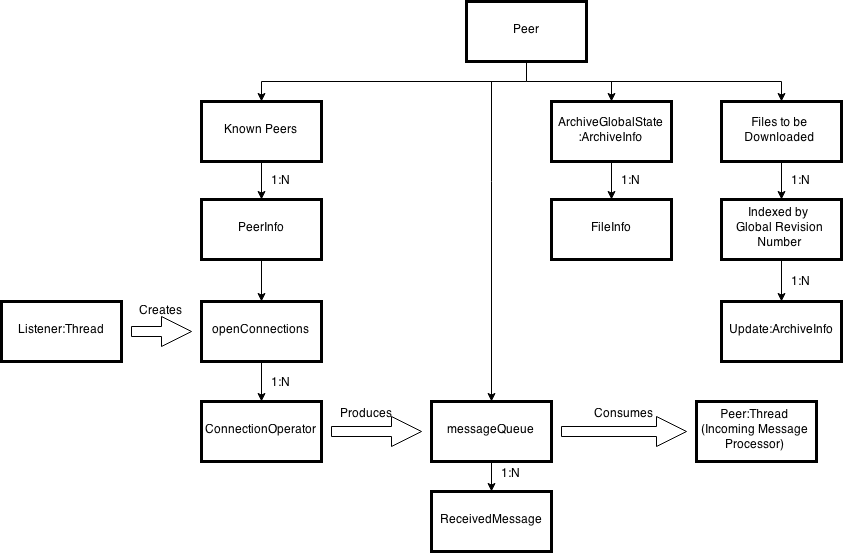
\includegraphics{strucs.png}
\caption{Figure 1: Main Program Data Structures}
\end{figure}

\sout{Really important implemented algorithms may be included (maybe in
the form of pseudocode), but do not include actual code, except for very
small portions of code that represent a solution to a particularly
interesting or difficult problem (even then, pseudocode is better).
Again, use figures as appropriate, e.g., to support discussion of
communication between main procedures/methods in terms of
procedure/method name, parameters, result type, function, relationship
to other procedures/methods and so on.}

\section{The system in operation/Process
description}\label{the-system-in-operationprocess-description}

\section{Common Scenarios}\label{common-scenarios}

\subsection{Definitions}\label{definitions}

\begin{description}
\item[P]
the publisher
\item[S]
a new subscriber
\end{description}

\subsection{Peer Starts Program Up (Not First Time) AKA Old Subscriber
Joins
Network}\label{peer-starts-program-up-not-first-time-aka-old-subscriber-joins-network}

\begin{enumerate}
\def\labelenumi{\arabic{enumi}.}
\item
  Peer checks integrity of file tree by checking against stored values
  of size, name, checksum for every file
\item
\begin{verbatim}
  If there are discrepancies:
        and we're a Subscriber:
            see Subscriber Loses Some Or All of Local Copy.
        or if we're the Publisher:
            see Publisher Has Updates
    else no discrepancies:
        If we're a Subscriber:
            check with Publisher about new peers and file updates
        Or if we're the Publisher:
            check if any new Peers have joined via DHT or otherwise
\end{verbatim}
\end{enumerate}

\subsection{New Subscriber Joins
Network}\label{new-subscriber-joins-network}

\begin{enumerate}
\def\labelenumi{\arabic{enumi}.}
\itemsep1pt\parskip0pt\parsep0pt
\item
  New subscriber S connects to publisher P on P's listening port
\item
  P and S exchange version numbers; if they don't match, disconnect and
  warn users at P and S
\item
  P and S exchange UUIDs. These will later serve as keys, mapping to
  PeerInfo objects.
\item
  S sends P PeerInfo of itself, containing relevant info (see message
  binary spec)
\item
  P sends S a File Tree Status object, informing S of the latest
  versions
\item
  P sends S a PeerInfo List of the peers it knows about (hopefully all
  of them)
\item
  S Greets peers it heard about from P, sends File Requests for
  files/versions it doesn't have
\item
  Peers send back list of requested pieces they have/are able to send
\item
  S chooses best peer to download each file or piece from, based on
  speed or other metrics
\item
  Some kind of sanity check is performed to make sure everything went OK
\end{enumerate}

\subsection{Publisher Has Updates to Push to All Subscribers / Publisher
Adds
Files}\label{publisher-has-updates-to-push-to-all-subscribers-publisher-adds-files}

\begin{enumerate}
\def\labelenumi{\arabic{enumi}.}
\itemsep1pt\parskip0pt\parsep0pt
\item
  P announces to all known peers the changed file revision numbers
  (partial fileTree state info)
\item
  If P has any data about bandwidths of various subscribers, the files
  are sent to the fastest first, to mazimise the number of peers that
  can supply the file. If not, a random subscriber is chosen
\item
  Every time a subscriber finishes downloading a file, it announces to
  peers it hasn't heard the same announcement from.
\item
  For every subscriber still downloading the file, requests are made for
  that file to those who have it.
\item
  Data is gathered by every peer about speeds during the transfer
\end{enumerate}

\subsection{Subscriber Leaves Network
Gracefully}\label{subscriber-leaves-network-gracefully}

\begin{enumerate}
\def\labelenumi{\arabic{enumi}.}
\itemsep1pt\parskip0pt\parsep0pt
\item
  Exit announcement is made to all known peers
\item
  Any transfers this subscriber has in progress are finished, or if
  they'll take too long (which is how long?), cancelled
\item
  Sockets etc are closed
\item
  Peers set their record for this Peer as `offline'
\end{enumerate}

\subsection{Subscriber is in the Middle of Downloading a FileID, When a
New Version is
Announced}\label{subscriber-is-in-the-middle-of-downloading-a-fileid-when-a-new-version-is-announced}

\subsection{Publisher Leaves Network
Gracefully}\label{publisher-leaves-network-gracefully}

the publisher may intend for the files to remain static, so a new
publisher won't be elected unless (good\_reason). any new peer which
joins by contacting a peer will be brought up to date by the network
(version check, file list exchange, sync files with p2p) once (if) it's
implemented, peers may also find the network by DHT.

\subsection{Subscriber Disappears Without Saying
Goodbye}\label{subscriber-disappears-without-saying-goodbye}

\begin{enumerate}
\def\labelenumi{\arabic{enumi}.}
\itemsep1pt\parskip0pt\parsep0pt
\item
  Subscriber fails heartbeats on each peer individually; each per
  individually marks it as offline in its local peer list.
\end{enumerate}

\subsection{Publisher Disappears Without Saying
Goodbye}\label{publisher-disappears-without-saying-goodbye}

\subsection{Subscriber loses some or all of local copy, subscriber
erroneously edits local
copy}\label{subscriber-loses-some-or-all-of-local-copy-subscriber-erroneously-edits-local-copy}

\begin{enumerate}
\def\labelenumi{\arabic{enumi}.}
\itemsep1pt\parskip0pt\parsep0pt
\item
  The user is warned that this is a bad idea: any changes will be
  overwritten. If they want to edit the files, then they should make a
  copy
\item
  Procedure for 1 out-of-date peer is followed
\item
  Request more peers and files from all known peers
\item
  Subscriber announces its loss
\end{enumerate}

\subsection{publisher loses its files}\label{publisher-loses-its-files}

\subsubsection{publisher loses its files while network has differing
versions
unresolved}\label{publisher-loses-its-files-while-network-has-differing-versions-unresolved}

situation is resolved by using file revision numbers (every update or
transaction if given a number, so with conflicting updates, the later
number will take priority) to bring all peers, including the Publisher,
up-to-date

\begin{enumerate}
\def\labelenumi{\arabic{enumi}.}
\itemsep1pt\parskip0pt\parsep0pt
\item
  Peers exchange information about the latest updates the've seen, until
  they are all in agreement.
\item
  updates which conflict are weeded out, and a list of updates which
  need applying to the network is created
\item
  Peers which have part or all of this update send what they have to
  everyone else
\end{enumerate}

\subsection{Complex states with no intuitive
solution}\label{complex-states-with-no-intuitive-solution}

\begin{itemize}
\itemsep1pt\parskip0pt\parsep0pt
\item
  a token, key or password is used by a peer to become the new publisher
  (P2)
\item
  Another peer becomes the publisher P2 while the old publisher (P1) is
  propagating updates
\item
  subscriber checks (with publisher or publisher-checked peers) that
  files are up-to-date
\item
  Publisher can't access a subscriber, but others can

  \begin{itemize}
  \itemsep1pt\parskip0pt\parsep0pt
  \item
    From the perspective of this weakly-connected peer S, the publisher
    is down
  \item
    From the publisher's perspective, the peer has disappeared without
    saying goodbye (timed out)
  \end{itemize}
\end{itemize}

There are common procedure to follow for some of these events:

\subsubsection{Generalisation: One Out-Of-Date
Peer}\label{generalisation-one-out-of-date-peer}

For example:

\begin{itemize}
\itemsep1pt\parskip0pt\parsep0pt
\item
  new peer joins network
\item
  peer loses its files (they are deleted, disk corrupt etc)
\item
  subscriber erroneously edits files
\end{itemize}

\paragraph{Procedure:}\label{procedure}

\begin{enumerate}
\def\labelenumi{\arabic{enumi}.}
\itemsep1pt\parskip0pt\parsep0pt
\item
  Out of date Peer P asks the publisher for the current revision number
  for every file in the tree, along with their checksums, size, and
  names
\item
  P asks all known peers for more peers (in case its local peer list has
  been partially or wholly corrupted), and files (filtering any which
  aren't as high
\end{enumerate}

(Note: possibly two chapters):

\sout{Give the reader a feel for what the system is like to use (this
may only be really relevant if the system has a user interface). Use
screen dumps to illustrate - textually quite a short chapter, maybe just
a walkthrough of the main features of a typical session with the system.
Note that this is not a user manual. You aren't showing the reader how
to operate the system, but rather what it's like to use. As a separate
chapter, you may also need a process description of your system, so that
the reader can appreciate how the system works. This is not the same as
the ``walkthrough'' described immediately above. It should be a
description at a higher level than the code itself. Use supporting
process diagrams as appropriate If your system has a significant user
interface and a complex underlying system you may need both a
walkthrough and a process chapter.}

\chapter{Testing \& Evaluation}\label{testing-evaluation}

\sout{How you evaluated the system, how you designed the evaluation.}

The main competitors to to this software are Bit-Torrent Sync and
Dropbox, due to the similarity of their technology compared to this
project. Although the primary intended use of this software is for
backup, these technological similarities along with the popularity of
Dropbox will mean they will offer direct competition.

\begin{itemize}
\itemsep1pt\parskip0pt\parsep0pt
\item
  Is the system user-friendly?
\item
  Is the system cross-platform?

  \begin{itemize}
  \itemsep1pt\parskip0pt\parsep0pt
  \item
    HOW cross platform? (Linux, Windows, Android\ldots{})
  \end{itemize}
\item
  Is the system resistant to attack?

  \begin{itemize}
  \itemsep1pt\parskip0pt\parsep0pt
  \item
    random peers going down
  \item
    Publisher impersonation/spoofing
  \item
    archive status misinformation
  \end{itemize}
\item
  How well does the system cope with sudden changes in network topology?
\item
  How efficient is it? (bandwidth usage, processor \& memory usage)
\item
  completeness of the API

  \begin{itemize}
  \itemsep1pt\parskip0pt\parsep0pt
  \item
    lack of ambiguity
  \end{itemize}
\end{itemize}

\section{Results of the evaluation}\label{results-of-the-evaluation}

\begin{itemize}
\itemsep1pt\parskip0pt\parsep0pt
\item
  \sout{A critical review of the evaluation itself}
\item
  \sout{how well it yielded the info you wanted.}
\end{itemize}

\sout{There may be a need to have two chapters, one on testing and one
on evaluation. Testing is intended to establish that the system
functions correctly. Evaluation examines how well the system achieves
its aim.}

\sout{For a system that features a user interface, some kind of user
interface evaluation is very important. For testing and evaluation, you
must include descriptions of the methodology and metrics used. Tables of
results may be included (main results can be summarised if a large
amount of test data was accumulated). Make sure you discuss interesting
and important results indicated by the data. Make sure you summarise
your overall findings, including statistical evaluation, and describing
methods.}

\chapter{Conclusions}\label{conclusions}

\sout{VERY important chapter. Revisit your objectives from chapter 1,
for each, analyse whether the project met that objective, and if not,
discuss this, and suggest a solution. Discuss the project as a whole, if
you did it again would you do it differently? What did you have to learn
to do the project, what did you learn from doing it? What features would
you add to your system if you had more time etc? Some suggested
subsections for your concluding chapter are: Review of aims; Suggested
revisions to design/implementation; Future work (possible developments
of existing system); Lessons learned. Finish the concluding chapter with
a brief, fairly upbeat overall conclusion on the project as a whole.
Even projects that are not an overall success usually achieve something,
and you acquire skills and knowledge from doing the project. End on a
positive note.}

\chapter{References}\label{references}

\end{document}
